\section{Depth-Based Tiebreaking for A*}

\label{sec:depth}

As shown in the previous section, the search spaces of Zerocost domains have many zero-cost edges,
resulting in a large final plateau ($\plateau{f^*,0}$). In a final plateau,
all nodes have $h=0$, so $h$-based tiebreaking cannot provide
useful guidance toward a goal. Thus, we need a new metric for discriminating among nodes
in the plateau so that the search algorithm can make progress in the plateau.

We define the \emph{depth} of a node as an 
integer representing the distance (number of steps) from the
\emph{entrance} of the plateau.  An \emph{entrance} of the plateau is
the first node which encountered in the plateau, along the path from the
initial node. These notions are depicted in
\refig{fig:plateau-depiction} (subfigure 1). 
Another way to think about depth is consider the problem of finding an exit from a particular plateau (i.e., finding either a goal node or exhausting the plateau) a unit-cost search space by itself -- the depth is analogous to a $g$-value for this space.
%It is equivalent to the $g$-value which is
%restricted to a particular plateau and is assuming the unit cost edges.

\begin{figure}[htbp]
  \centering
  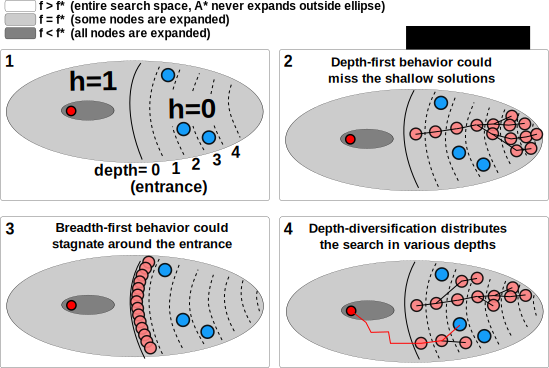
\includegraphics{img/astar/plateau-2.pdf}
 \caption{(\textbf{Subfigure 1}) The nodes in a plateau are divided into several layers, and each layer have the corresponding depth. Since all nodes have $f=f^*$, depth does not affect optimality. The goals in both shallower or deeper region yield cost-optimal solutions.
 (\textbf{Subfigure 2}) \lifo tiebreaking strategy results in depth-first behavior in a
 plateau, which could miss solutions if they are concentrated near the entrance.
 (\textbf{Subfigure 3}) \fifo tiebreaking strategy results in  breadth-first behavior in a
 plateau, which could fail to reach a solutions in deeper layers within the time limit.
 (\textbf{Subfigure 4}) Depth-based diversification allows \astar to search the plateau space
 sparsely in a less biased, more uniformly and manner. This balances exploration and exploitation, avoiding the problems with both \lifo (depth-first) and \fifo (breadth-first) behavior.
 }
 \label{fig:plateau-depiction}
\end{figure}

The depth $d(n)$ of a
node $n$ is 0 when $n$ and the parent node $m$ have different key
values for a sorting strategy, and $d(n)=d(m)+1$ when they have the same
key values: For example, in \astar with $h$-based tiebreaking, the key
values of a node are represented as a vector $[f,h]$, and they are same
when they are pairwise equivalent (i.e. $f(n) = f(m) \land h(n) =
h(m)$).  Having the same key values means that $n$ and $m$ are in the
same plateau.

The traditional \lifo and \fifo tiebreaking strategy 
search the plateau region in decreasing and increasing order of the depth, respectively.
The \lifo strategy always selects the most recently generated node
within $\plateau{f,h}$, and the behavior in the plateau is equivalent to depth-first search.
Thus, \lifo always selects the largest depth
buckets, as depicted in \refig{fig:plateau-depiction} (subfigure 2).
Similarly, the behavior of the \fifo strategy 
in a plateau is equivalent to breadth-first search. Thus \fifo 
always selects the nodes with least depth (subfigure 3).
Note that  $[f,h,\lifo]$ is equivalent to $[f,h,-d,\lifo]$ and
$[f,h,\fifo]$ is equivalent to $[f,h,d,\fifo]$.

The problem with these traditional strategies is that we have no knowledge
regarding whether the goals are located close to or far from the entrance. Recall
that since $f=f^*$, all goal nodes in the final plateau are optimal with respect to solution cost.
regardless of the depth.%: A goal node in a shallower region or a deeper region both yields a cost-optimal solution. 
However, until we find a
solution, we do not know how the goals are distributed among various
depths. In some problem instance the goals can be concentrated around
the entrance, and in other problem instances the goals can be
concentrated at some large depth. % $k$.  k never used below?

In the former case, (\fifo), whose breadth-first behavior naturally
focuses the search around the entrance favoring the smaller depths,
should perform well, but in the latter case, exhaustively searching
the shallower depths can result in not finding any solutions within
the time limit because \fifo may never reach the depth where the goals
exist.  On the other hand, \lifo behaves in a depth-fist manner, so it
may reach solutions at deeper depths quickly, but risks missing
solutions at shallower depths.  Thus, both \fifo and \lifo tiebreaking
are prone to failures due to pathological cases.

In order to avoid focusing the search at the wrong depths (too shallow/deep), 
the safest policy seems to be to simply \emph{diversify} the depths which are being searched,
in order to avoid any depth-based biases which could lead to pathological behavior.
In our proposed \emph{depth diversification} strategy, the nodes are inserted into buckets
associated with depths, and upon expansion, search effort is distributed in a more balanced manner
among various depths (\refsec{sec:theoretical-characteristics} defines ``more balanced''  more precisely).
Nodes are not  ``sorted''
according to increasing or decreasing order of depth -- instead we try to 
``diversify'' the node expansion within the plateau.
We denote this depth diversification criterion as $\depth$. 
For example, $[f,h,\depth]$ first breaks ties according to $h$ values,
then uses the $\depth$ criterion to break ties in $\plateau{f,h}$.
%We denote such a diversification family of
%tiebreaking strategies by enclosing it in brackets such as $[f,h,\depth]$.

In order to diversify the expansion among depths, we simply
iterate over the depth buckets. An index $d_c$,
 which stores the depth (bucket index)  which was selected in the last expansion,
is initialized to 0.
At each expansion, the counter is decremented ($d_c\leftarrow d_c-1$) and
a node from  bucket $d_c$ is expanded. When $d_c$ reaches below 0, then $d_c$
is reset to the current largest depth in the plateau.

In an earlier, conference paper, we used a non-deterministic,
randomized implementation of this idea \cite{Asai16}, but we use a deterministic
implementation here because it eliminates the possibility of results being influenced by random seeds,
and also facilitates the  theoretical analysis below in \refsec{sec:theoretical-characteristics}.

% We later show that
% \fifo and \lifo strategies are incomplete when the size of the plateau
% region is inifinite, while our \id is probabilistically complete.

\subsection{The Scope Captured by Depth-Based Tiebreaking}

% ``no effect'' is ambiguous, reviewers may complain that we are trying to claim there is no overhead, including the low level overhead. Thus I reworded from ``no effect'' to ``does not affect the order of expansion''.
Depth-based tiebreaking does not affect the order of node expansion when there are no remaining ties after the
higher priority tiebreaking criteria, in which case all nodes have depth 0. \todo*{mentioning ``keys'' seems
unnecessarily complicated, so remove it}
% 
This happens when the target problem only has operators with positive cost.
Let a node $n$ is a child of a node $m$. Depending on whether $n$ is already evaluated and whether the parent of $n$ is updated or not, there are 3 cases:

\begin{enumerate}
 \item If $n$ is evaluated for the first time,
       then $g(n)=g(m)+\mit{cost}(m,n) > g(m)$ and so $f(n)-h(n) > f(m)-h(m)$.
       Thus $f(n)=f(m)$ and $h(n)=h(m)$ cannot hold at the same time and the depth is 0.
 \item If $n$ is already evaluated as a child of another node $m'$, $n$'s current parent is $m'$ and
       $g(m)+\mit{cost}(m,n) < g(m') + \mit{cost}(m',n) = g(n)$,
       then the parent of $n$ is updated to $m$ and $g(n)\leftarrow g(m)+\mit{cost}(m,n)$.
       Since $g(n)=g(m)+\mit{cost}(m,n)>g(m)$ and so $f(n)-h(n) > f(m)-h(m)$,
       therefore $f(n)=f(m)$ and $h(n)=h(m)$ cannot hold at the same time and the depth is 0.
 \item If $n$ is already evaluated as a child of another node $m'$, $n$'s current parent is $m'$ and
       $g(m)+\mit{cost}(m,n) \geq g(m') + \mit{cost}(m',n) = g(n)$, then the parent of $n$ remains $m'$. If the
       depth of $n$ is 0 at this moment, then it remains 0 because the parent is unchanged.
\end{enumerate}

Since the case 1 and 2 always hold and the case 3 holds at the beginning of the search,
by mathematical induction, the case 3 always holds during the search.
Thus, the depths of nodes in positive cost domains are always 0.

\subsection{Tiebreaking within Depth Buckets}

Consider a tiebreaking strategy such as $[f,h,\depth]$ which applies a depth-diversification tiebreaking.
After the $\depth$ criterion is applied, 
there may be multiple nodes within the same depth bucket, so a
default tiebreaking criterion is still necessary to break ties among them.
Thus we should, for example, apply one of \lifo, \fifo or \ro (random order) criteria
after $\depth$ criterion.

There could be still a room for heuristic-agnostic improvements between $\depth$ and default criterion,
\todo*{``this level'' == after $\depth$} while this is not in the scope of this paper.  For example, while depth
metric measures and diversifies the depth in a plateau, another criterion $X$ may non-trivially diversify the
search in a breadth direction before the default criterion, such as $[f,h,\depth,X,\fifo]$.

Candidates for $X$ may
include pruning techniques such as Symmetry Breaking \cite{Fox1998,pochter2011exploiting,domshlak2013symmetry} or
Partial Order Reduction \cite{hall2013faster,wehrle2013relative}.
While they are usually described as ``pruning techniques'',
they can be rephrased as ``removing the bias to a particular set
of nodes which shares the same characteristics'' because they both aim to
prune the redundant nodes. Note that redundancy causes a biased 
search effort. For example, imagine we have a
set of nodes $S=\{a_1, a_2, a_3, a_4, b, c, d\}$ where
$A=\{a_1, a_2, a_3, a_4\}$ are ``redundant'' in some measure (e.g. by Symmetry,
Partial-Order). 
If a search algorithm expands $S$ by random selection, it favors the
group $A$ by giving a 4 times larger chance of expansion than $b$,
$c$ or $d$.

% \todo{compare id,fifo and id,lifo}
CommentOnTheDeletedActionOrderingText\todo{Although there's no need to show new results for action ordering, 
it may be a good idea to summarize+point to the AAAI16 action ordering experiment, in order to eliminate concerns that
all our results are somehow specific to one particular action order.}
% However we use a Random Order (\ro) criterion, which 
% randomly selects an element from the depth bucket selected by the depth-based tiebreaking.
% This is because the effectiveness of the tiebreaking behavior within a bucket
% can be affected by accidental biases, e.g., names/orders of action schema in the PDDL domain
% definition \cite{vallati2015effective}.
% %Finding the best action ordering is not the scope of this paper.
% Thus, we avoid bias at this level of tiebreaking by using \ro and assess its expected/average
% performance.

% Among \fifo, \lifo and \ro, the natural criterion is Random Order.
% This is because the effectiveness of the third-level tiebreaking behavior
% is affected by the accidental bias in action ordering in the PDDL domain
% definition.  Recent work \cite{vallati2015effective} showed that the
% planner performance is greatly affected by changing and tuning the action ordering
% (and also variable ordering, but it is irrelevant to the tiebreaking behavior). 
% However, finding the best third-level tiebreaking is not the scope of this paper.
% Thus, focusing on \ro and assess its expected/average
% performance is the most reasonable practice to understand the behavior of second-level,
% depth-based tiebreaking.

\subsection{Theoretical Characteristics of the Depth Distribution}
\label{sec:theoretical-characteristics}

We give further insight into the search behavior of our implementation
of depth-based diversification.
As described above, our implementation performs a deterministic, round-robin sampling from the available depth buckets.
%iterates from the largest depth to 0.

%We are particularly interested in how the expansions happen among the
%various depths in the plateau region.
We are particularly interested in how the nodes selected for expansion are distributed 
among the various depths in a plateau region.
Using a simplified model where the plateau region is a tree,
we show that the probability of expanding a node in a particular depth
can be represented by a simple formula.  Although the notion of
probability does not fit well with deterministic \fifo or \lifo
default tiebreaking, it is meaningful in the case of \ro (random
order) default tiebreaking.

%% danger!!
% \begin{theo}[Uniformness of the search]
%  Assume the search space forms a tree of fixed width $w\geq 2$.
%  After enough number of iterations $D$,
%  the chance of expanding each node is unaffected by the depth of the
%  node, if the depth $d$ is small relative to $D$.
% \end{theo}

% I no longer claim the distribution is uniform.
As a preparation, we first show that the number of expansion happened to each depth decreases
linearly to the depth.
% 
\todo*{Introduced the tree assumption in the beginning.}
We first assume that the plateau region form a tree of a fixed branching factor
$w\geq 2$ (\emph{tree assumption}), rather than a graph with indefinite number of successor nodes.
We also assume that no depth buckets exhaust due to the expansion (\emph{no-exhaust assumption}).

Let $D\geq 0$ be the current largest depth of the nodes found in the plateau so far.  If the expansion of a node in
depth $D$ resulted in more nodes in the same plateau, then the children have depth $D+1$.  Due to the tree
assumption, these children are all newly generated. Also, as we explained in the previous section, the expansion is
diversified by a sequence of iterations from the current largest depth to 0.  It means that when the current
largest depth of the plateau is $D$, the number of iteration happened so far is also $D$.
% Under the tree assumption, each expansion of depth $d$ results in $w$ new nodes in depth $d+1$. 
Therefore, at the end of the $D$'th iteration, each depth $d$ has been expanded exactly $D-d$ times, with $D(D-1)$
expansions in total.

It also means that the minimum condition for \emph{no-exhaust assumption} to hold until the end of the $D$'th
iteration is that the initial number of nodes in depth 0 is at least $D$.  If there are at least $D$ nodes in depth
0, depth 0 trivially never exhausts until $D$'th iteration. Also, no depth buckets in depth $d>0$ will exhaust
because each bucket have $w^{D-d-1}$ nodes in total (including those already expanded) while the expansion has
happened only $D-d$ times. For simplicity, let us also assume that the depth 0 initially have exactly $D$ nodes and
no nodes will be added to depth 0 during the search.

Now we show the formula which represents the probability of expanding a node in a particular depth.
At the end of $D$'th iteration,
each depth $d-1$ is expanded $D-(d-1)$ times in the preceding $D$ iterations.
Therefore, the total number of nodes that have been in depth $d$, including those
that have been expanded so far, is $w(D-d+1)$.
Expansion has happened $D(D-1)$ times in total, and depth $d$ is expanded $D-d$ times.
Thus, the probability of expanding each node in depth $d$ is
$\frac{D-d}{D(D-1)\cdot w(D-d+1)}=\frac{1}{wD(D-1)}(1-\frac{1}{D-d+1})$.  \qed

Notice that $\frac{1}{D-d+1}$ is negligible if $D \gg d$.
Thus, after enough number of iterations (large $D$), the nodes are 
expanded in an approximately equal probability $\frac{1}{wD(D-1)}$ in the shallower region, and is
unaffected by the depth of the node.
However, the nodes near the largest depth has less probability, showing
some balance in exploration and exploitation.

The important point of this characteristics is that this distribution is maintained at any point of the search
until the solution is found. In fact, any depth-selection criterion, including the least depth selection (\fifo) or
the largest depth selection (\lifo), result in the same distribution if all nodes are to be expanded (each depth
$d$ is expanded $Dw^d$ times), but their online characteristics are not.
%
\todo*{maybe \lifo and \fifo should be analyzed wrto this tree model and compared directly to each other as well as
$\depth$?}
\todo*{less priority -- lets add it when required by the reviewers. unused texts are in unused/lifo-fifo-distribution.tex}
